%%%%%%%%%%%%%%%%%%%%%%%%%%%%%%%%%%%%%%%%%%%%%%%%%%%%%%%%%%%%%%%%%%%%%%%%%%%%%%%%%%%%%%%%%%%%%%%%%%%
%%%%%%%%%%%%%%%%%%%%%%%%%%%%%%%%%%%%%%%%%%%%%%%%%%%%%%%%%%%%%%%%%%%%%%%%%%%%%%%%%%%%%%%%%%%%%%%%%%%
\chapter{Tablas y gr\'aficos}

En este ap\'endice se incluyen las gr\'aficas y tablas obtenidas durante el trabajo; en las 
diferentes secciones del texto 
puede hallarse una descripci\'on m\'as extensa de las tablas a aocontinucai\'on, c\'omo se
calcularon y que significan, as\'i algunas posibles interpretaciones.

%%%%%%%%%%%%%%%%%%%%%%%%%%%%%%%%%%%%%%%%%%%%%%%%%

\begin{SidewaysFigure}
\centering
\begin{tabular}{c|ccccc|cccc|ccc}
& VCR & MJH & JAE & GHA & MFGR
& CLO & RLO & RRU & JGZ
& FGH & MGG & EMT \\
\hline
C3&68&18&10&40&106&6&35&45&1&2&28&9 \\
C4&58&16&4&32&97&4&40&49&0&1&23&10 \\
CZ&46&16&13&37&89&5&22&39&1&1&13&12 \\
F3&62&23&10&10&64&7&43&39&3&6&14&4 \\
F4&55&23&5&20&51&6&36&34&0&0&4&15 \\
F7&41&15&2&24&48&1&18&9&0&0&2&2 \\
F8&57&11&6&13&32&4&23&6&0&0&2&11 \\
FP1&30&7&1&6&41&0&0&10&0&22&0&8 \\
FP2&41&6&3&13&24&1&15&6&0&0&1&4 \\
FZ&67&18&19&11&67&7&38&41&2&0&20&14 \\
O1&100&20&5&4&121&2&25&54&2&5&18&13 \\
O2&85&23&3&12&121&3&34&43&1&1&12&5 \\
P3&74&17&2&23&123&5&33&41&0&1&24&11 \\
P4&66&19&4&29&117&4&27&46&1&4&15&11 \\
PZ&71&15&5&32&117&4&32&41&0&1&8&7 \\
T3&79&29&1&19&115&10&34&33&0&2&29&7 \\
T4&73&20&2&26&104&3&35&44&1&0&10&13 \\
T5&85&26&0&4&121&5&34&41&2&2&31&15 \\
T6&76&18&3&20&120&3&24&46&2&0&9&11 \\
LOG&33&20&8&14&68&5&11&13&0&1&8&13 \\
ROG&36&21&17&9&77&9&7&18&1&0&19&16 \\
EMG&74&11&0&1&97&14&16&18&0&0&3&1 \\
\hline
Total&200&127&171&134&267&132&99&114&33&22&166&47
\end{tabular}
\caption{Total de \'epocas PE clasificadas como sue\~no MOR 
(fase R) para cada
canal. %Se incluyen las medias y desviaciones est\'andar estimadas para los grupos 
%Control (izquierda) y PDC (centro).
}
\label{total_gpos_mor}
\end{SidewaysFigure}

\begin{SidewaysFigure}
\centering
\begin{tabular}{c|ccccc|cccc|ccc}
& VCR & MJH & JAE & GHA & MFGR
& CLO & RLO & RRU & JGZ
& FGH & MGG & EMT \\
\hline
C3&696&135&100&970&635&55&153&324&56&16&201&72 \\
C4&700&129&89&980&551&36&135&367&47&7&207&92 \\
CZ&675&131&88&878&503&54&145&324&62&8&180&70 \\
F3&674&134&83&800&496&57&175&293&68&107&143&46 \\
F4&677&132&55&936&381&41&135&287&49&0&137&91 \\
F7&616&137&77&781&545&45&112&268&58&0&152&40 \\
F8&672&123&30&894&421&41&96&303&48&0&128&92 \\
FP1&551&75&23&779&462&34&0&250&44&381&169&72 \\
FP2&613&82&44&898&341&33&99&186&44&0&146&56 \\
FZ&661&134&78&930&513&55&163&293&65&0&177&87 \\
O1&797&174&51&410&871&48&150&380&96&20&140&123 \\
O2&785&165&63&659&874&32&136&327&106&22&161&106 \\
P3&756&122&53&863&736&72&147&364&95&29&212&66 \\
P4&763&136&108&959&633&56&135&366&73&18&206&73 \\
PZ&723&131&90&862&593&57&167&361&59&15&177&65 \\
T3&688&140&52&509&691&81&112&290&102&27&115&89 \\
T4&763&121&35&956&693&26&110&358&87&10&122&70 \\
T5&826&146&16&455&843&78&137&378&61&19&208&109 \\
T6&790&148&49&747&829&38&118&348&84&18&209&119 \\
LOG&684&224&214&1124&759&144&185&376&225&50&437&179 \\
ROG&674&205&212&1156&789&126&179&321&225&67&455&210 \\
EMG&718&62&16&19&785&20&82&321&10&1&55&42 \\
\hline
Total&2384&905&736&3147&2199&812&747&1130&1174&383&864&508
\end{tabular}
\caption{Total  de \'epocas PE dentro del registro pero que no fueron clasificadas
como MOR (fases W y N) para cada
canal. %Se incluyen las medias y desviaciones est\'andar estimadas para los grupos 
%Control (izquierda) y PDC (centro).
}
\label{total_gpos_nmor}
\end{SidewaysFigure}

\begin{SidewaysFigure}
\centering
\begin{tabular}{c|ccccc|cccc|ccc}
& VCR & MJH & JAE & GHA & MFGR
& CLO & RLO & RRU & JGZ
& FGH & MGG & EMT \\
\hline
C3&764&153&110&1010&741&61&188&369&57&18&229&81 \\
C4&758&145&93&1012&648&40&175&416&47&8&230&102 \\
CZ&721&147&101&915&592&59&167&363&63&9&193&82 \\
F3&736&157&93&810&560&64&218&332&71&113&157&50 \\
F4&732&155&60&956&432&47&171&321&49&0&141&106 \\
F7&657&152&79&805&593&46&130&277&58&0&154&42 \\
F8&729&134&36&907&453&45&119&309&48&0&130&103 \\
FP1&581&82&24&785&503&34&0&260&44&403&169&80 \\
FP2&654&88&47&911&365&34&114&192&44&0&147&60 \\
FZ&728&152&97&941&580&62&201&334&67&0&197&101 \\
O1&897&194&56&414&992&50&175&434&98&25&158&136 \\
O2&870&188&66&671&995&35&170&370&107&23&173&111 \\
P3&830&139&55&886&859&77&180&405&95&30&236&77 \\
P4&829&155&112&988&750&60&162&412&74&22&221&84 \\
PZ&794&146&95&894&710&61&199&402&59&16&185&72 \\
T3&767&169&53&528&806&91&146&323&102&29&144&96 \\
T4&836&141&37&982&797&29&145&402&88&10&132&83 \\
T5&911&172&16&459&964&83&171&419&63&21&239&124 \\
T6&866&166&52&767&949&41&142&394&86&18&218&130 \\
LOG&717&244&222&1138&827&149&196&389&225&51&445&192 \\
ROG&710&226&229&1165&866&135&186&339&226&67&474&226 \\
EMG&792&73&16&20&882&34&98&339&10&1&58&43 \\
\hline
Total&2584&1032&907&3281&2466&944&846&1244&1207&405&1030&555
\end{tabular}
\caption{Total de \'epocas PE registradas
(todas las fases) para cada
canal. 
%Se incluyen las medias y desviaciones est\'andar estimadas para los grupos 
%Control (izquierda) y PDC (centro).
}
\label{total_gpos_total}
\end{SidewaysFigure}






%\begin{comment}
\begin{SidewaysFigure}
\centering
\begin{tabular}{c||ccccc|cc||cccc|cc||ccc}
& VCR & MJH & JAE & GHA & MFGR &$\widehat{\mu}$ & $\widehat{\sigma}$
& CLO & RLO & RRU & JGZ &$\widehat{\mu}$ & $\widehat{\sigma}$
& FGH & MGG & EMT \\
\hline
 C3 & 0.340    & 0.142    & 0.058    & 0.299    & 0.397    & 0.247    & 0.142    & 0.045    & 0.354    & 0.395    & 0.030    & 0.206    & 0.195    & 0.091    & 0.169    & 0.191     \\
 C4 & 0.290    & 0.126    & 0.023    & 0.239    & 0.363    & 0.208    & 0.135    & 0.030    & 0.404    & 0.430    & -      & 0.216    & 0.233    & 0.045    & 0.139    & 0.213     \\
 CZ & 0.230    & 0.126    & 0.076    & 0.276    & 0.333    & 0.208    & 0.106    & 0.038    & 0.222    & 0.342    & 0.030    & 0.158    & 0.151    & 0.045    & 0.078    & 0.255     \\
 F3 & 0.310    & 0.181    & 0.058    & 0.075    & 0.240    & 0.173    & 0.107    & 0.053    & 0.434    & 0.342    & 0.091    & 0.230    & 0.187    & 0.273    & 0.084    & 0.085     \\
 F4 & 0.275    & 0.181    & 0.029    & 0.149    & 0.191    & 0.165    & 0.089    & 0.045    & 0.364    & 0.298    & -      & 0.177    & 0.181    & -      & 0.024    & 0.319     \\
 F7 & 0.205    & 0.118    & 0.012    & 0.179    & 0.180    & 0.139    & 0.078    & 0.008    & 0.182    & 0.079    & -      & 0.067    & 0.084    & -      & 0.012    & 0.043     \\
 F8 & 0.285    & 0.087    & 0.035    & 0.097    & 0.120    & 0.125    & 0.095    & 0.030    & 0.232    & 0.053    & -      & 0.079    & 0.105    & -      & 0.012    & 0.234     \\
 FP1 & 0.150    & 0.055    & 0.006    & 0.045    & 0.154    & 0.082    & 0.066    & -      & -      & 0.088    & -      & 0.022    & 0.044    & 1.000    & -      & 0.170     \\
 FP2 & 0.205    & 0.047    & 0.018    & 0.097    & 0.090    & 0.091    & 0.071    & 0.008    & 0.152    & 0.053    & -      & 0.053    & 0.070    & -      & 0.006    & 0.085     \\
 FZ & 0.335    & 0.142    & 0.111    & 0.082    & 0.251    & 0.184    & 0.106    & 0.053    & 0.384    & 0.360    & 0.061    & 0.214    & 0.182    & -      & 0.120    & 0.298     \\
 O1 & 0.500    & 0.157    & 0.029    & 0.030    & 0.453    & 0.234    & 0.228    & 0.015    & 0.253    & 0.474    & 0.061    & 0.200    & 0.209    & 0.227    & 0.108    & 0.277     \\
 O2 & 0.425    & 0.181    & 0.018    & 0.090    & 0.453    & 0.233    & 0.197    & 0.023    & 0.343    & 0.377    & 0.030    & 0.193    & 0.193    & 0.045    & 0.072    & 0.106     \\
 P3 & 0.370    & 0.134    & 0.012    & 0.172    & 0.461    & 0.230    & 0.182    & 0.038    & 0.333    & 0.360    & -      & 0.183    & 0.190    & 0.045    & 0.145    & 0.234     \\
 P4 & 0.330    & 0.150    & 0.023    & 0.216    & 0.438    & 0.232    & 0.160    & 0.030    & 0.273    & 0.404    & 0.030    & 0.184    & 0.186    & 0.182    & 0.090    & 0.234     \\
 PZ & 0.355    & 0.118    & 0.029    & 0.239    & 0.438    & 0.236    & 0.167    & 0.030    & 0.323    & 0.360    & -      & 0.178    & 0.189    & 0.045    & 0.048    & 0.149     \\
 T3 & 0.395    & 0.228    & 0.006    & 0.142    & 0.431    & 0.240    & 0.177    & 0.076    & 0.343    & 0.289    & -      & 0.177    & 0.165    & 0.091    & 0.175    & 0.149     \\
 T4 & 0.365    & 0.157    & 0.012    & 0.194    & 0.390    & 0.224    & 0.156    & 0.023    & 0.354    & 0.386    & 0.030    & 0.198    & 0.199    & -      & 0.060    & 0.277     \\
 T5 & 0.425    & 0.205    & -      & 0.030    & 0.453    & 0.223    & 0.213    & 0.038    & 0.343    & 0.360    & 0.061    & 0.200    & 0.175    & 0.091    & 0.187    & 0.319     \\
 T6 & 0.380    & 0.142    & 0.018    & 0.149    & 0.449    & 0.228    & 0.180    & 0.023    & 0.242    & 0.404    & 0.061    & 0.182    & 0.176    & -      & 0.054    & 0.234     \\
 LOG & 0.165    & 0.157    & 0.047    & 0.104    & 0.255    & 0.146    & 0.077    & 0.038    & 0.111    & 0.114    & -      & 0.066    & 0.056    & 0.045    & 0.048    & 0.277     \\
 ROG & 0.180    & 0.165    & 0.099    & 0.067    & 0.288    & 0.160    & 0.085    & 0.068    & 0.071    & 0.158    & 0.030    & 0.082    & 0.054    & -      & 0.114    & 0.340     \\
 EMG & 0.370    & 0.087    & -      & 0.007    & 0.363    & 0.165    & 0.187    & 0.106    & 0.162    & 0.158    & -      & 0.106    & 0.075    & -      & 0.018    & 0.021    
\end{tabular}
\caption{Proporci\'on estimada de \'epocas PE respecto al total de \'epocas MOR 
(fase R) para cada
canal. Se incluyen las medias y desviaciones est\'andar estimadas para los grupos 
Control (izquierda) y PDC (centro).}
\label{gpos_mor}
\end{SidewaysFigure}

\begin{SidewaysFigure}
\centering
\begin{tabular}{c||ccccc|cc||cccc|cc||ccc}
& VCR & MJH & JAE & GHA & MFGR &$\widehat{\mu}$ & $\widehat{\sigma}$
& CLO & RLO & RRU & JGZ &$\widehat{\mu}$ & $\widehat{\sigma}$
& FGH & MGG & EMT \\
\hline
 C3 & 0.292    & 0.149    & 0.136    & 0.308    & 0.289    & 0.235    & 0.085    & 0.068    & 0.205    & 0.287    & 0.048    & 0.152    & 0.114    & 0.042    & 0.233    & 0.142     \\
 C4 & 0.294    & 0.143    & 0.121    & 0.311    & 0.251    & 0.224    & 0.087    & 0.044    & 0.181    & 0.325    & 0.040    & 0.147    & 0.135    & 0.018    & 0.240    & 0.181     \\
 CZ & 0.283    & 0.145    & 0.120    & 0.279    & 0.229    & 0.211    & 0.076    & 0.067    & 0.194    & 0.287    & 0.053    & 0.150    & 0.111    & 0.021    & 0.208    & 0.138     \\
 F3 & 0.283    & 0.148    & 0.113    & 0.254    & 0.226    & 0.205    & 0.072    & 0.070    & 0.234    & 0.259    & 0.058    & 0.155    & 0.106    & 0.279    & 0.166    & 0.091     \\
 F4 & 0.284    & 0.146    & 0.075    & 0.297    & 0.173    & 0.195    & 0.095    & 0.050    & 0.181    & 0.254    & 0.042    & 0.132    & 0.103    & -      & 0.159    & 0.179     \\
 F7 & 0.258    & 0.151    & 0.105    & 0.248    & 0.248    & 0.202    & 0.070    & 0.055    & 0.150    & 0.237    & 0.049    & 0.123    & 0.089    & -      & 0.176    & 0.079     \\
 F8 & 0.282    & 0.136    & 0.041    & 0.284    & 0.191    & 0.187    & 0.103    & 0.050    & 0.129    & 0.268    & 0.041    & 0.122    & 0.105    & -      & 0.148    & 0.181     \\
 FP1 & 0.231    & 0.083    & 0.031    & 0.248    & 0.210    & 0.161    & 0.097    & 0.042    & -      & 0.221    & 0.037    & 0.075    & 0.099    & 0.995    & 0.196    & 0.142     \\
 FP2 & 0.257    & 0.091    & 0.060    & 0.285    & 0.155    & 0.170    & 0.099    & 0.041    & 0.133    & 0.165    & 0.037    & 0.094    & 0.065    & -      & 0.169    & 0.110     \\
 FZ & 0.277    & 0.148    & 0.106    & 0.296    & 0.233    & 0.212    & 0.082    & 0.068    & 0.218    & 0.259    & 0.055    & 0.150    & 0.104    & -      & 0.205    & 0.171     \\
 O1 & 0.334    & 0.192    & 0.069    & 0.130    & 0.396    & 0.224    & 0.137    & 0.059    & 0.201    & 0.336    & 0.082    & 0.169    & 0.127    & 0.052    & 0.162    & 0.242     \\
 O2 & 0.329    & 0.182    & 0.086    & 0.209    & 0.397    & 0.241    & 0.123    & 0.039    & 0.182    & 0.289    & 0.090    & 0.150    & 0.110    & 0.057    & 0.186    & 0.209     \\
 P3 & 0.317    & 0.135    & 0.072    & 0.274    & 0.335    & 0.227    & 0.117    & 0.089    & 0.197    & 0.322    & 0.081    & 0.172    & 0.113    & 0.076    & 0.245    & 0.130     \\
 P4 & 0.320    & 0.150    & 0.147    & 0.305    & 0.288    & 0.242    & 0.086    & 0.069    & 0.181    & 0.324    & 0.062    & 0.159    & 0.123    & 0.047    & 0.238    & 0.144     \\
 PZ & 0.303    & 0.145    & 0.122    & 0.274    & 0.270    & 0.223    & 0.083    & 0.070    & 0.224    & 0.319    & 0.050    & 0.166    & 0.128    & 0.039    & 0.205    & 0.128     \\
 T3 & 0.289    & 0.155    & 0.071    & 0.162    & 0.314    & 0.198    & 0.101    & 0.100    & 0.150    & 0.257    & 0.087    & 0.148    & 0.077    & 0.070    & 0.133    & 0.175     \\
 T4 & 0.320    & 0.134    & 0.048    & 0.304    & 0.315    & 0.224    & 0.126    & 0.032    & 0.147    & 0.317    & 0.074    & 0.143    & 0.126    & 0.026    & 0.141    & 0.138     \\
 T5 & 0.346    & 0.161    & 0.022    & 0.145    & 0.383    & 0.211    & 0.151    & 0.096    & 0.183    & 0.335    & 0.052    & 0.166    & 0.125    & 0.050    & 0.241    & 0.215     \\
 T6 & 0.331    & 0.164    & 0.067    & 0.237    & 0.377    & 0.235    & 0.125    & 0.047    & 0.158    & 0.308    & 0.072    & 0.146    & 0.118    & 0.047    & 0.242    & 0.234     \\
 LOG & 0.287    & 0.248    & 0.291    & 0.357    & 0.345    & 0.306    & 0.045    & 0.177    & 0.248    & 0.333    & 0.192    & 0.237    & 0.070    & 0.131    & 0.506    & 0.352     \\
 ROG & 0.283    & 0.227    & 0.288    & 0.367    & 0.359    & 0.305    & 0.059    & 0.155    & 0.240    & 0.284    & 0.192    & 0.218    & 0.056    & 0.175    & 0.527    & 0.413     \\
 EMG & 0.301    & 0.069    & 0.022    & 0.006    & 0.357    & 0.151    & 0.165    & 0.025    & 0.110    & 0.284    & 0.009    & 0.107    & 0.126    & 0.003    & 0.064    & 0.083    
\end{tabular}
\caption{Proporci\'on estimada de \'epocas PE respecto al total de \'epocas no-MOR 
(fases W y N) para cada
canal. Se incluyen las medias y desviaciones est\'andar estimadas para los grupos 
Control (izquierda) y PDC (centro).}
\label{gpos_nmor}
\end{SidewaysFigure}

\begin{SidewaysFigure}
\centering
\begin{tabular}{c||ccccc|cc||cccc|cc||ccc}
& VCR & MJH & JAE & GHA & MFGR &$\widehat{\mu}$ & $\widehat{\sigma}$
& CLO & RLO & RRU & JGZ &$\widehat{\mu}$ & $\widehat{\sigma}$
& FGH & MGG & EMT \\
\hline
 C3 & 0.296    & 0.148    & 0.121    & 0.308    & 0.300    & 0.235    & 0.092    & 0.065    & 0.222    & 0.297    & 0.047    & 0.158    & 0.122    & 0.044    & 0.222    & 0.146     \\
 C4 & 0.293    & 0.141    & 0.103    & 0.308    & 0.263    & 0.222    & 0.094    & 0.042    & 0.207    & 0.334    & 0.039    & 0.156    & 0.143    & 0.020    & 0.223    & 0.184     \\
 CZ & 0.279    & 0.142    & 0.111    & 0.279    & 0.240    & 0.210    & 0.079    & 0.063    & 0.197    & 0.292    & 0.052    & 0.151    & 0.115    & 0.022    & 0.187    & 0.148     \\
 F3 & 0.285    & 0.152    & 0.103    & 0.247    & 0.227    & 0.203    & 0.074    & 0.068    & 0.258    & 0.267    & 0.059    & 0.163    & 0.115    & 0.279    & 0.152    & 0.090     \\
 F4 & 0.283    & 0.150    & 0.066    & 0.291    & 0.175    & 0.193    & 0.095    & 0.050    & 0.202    & 0.258    & 0.041    & 0.138    & 0.109    & -      & 0.137    & 0.191     \\
 F7 & 0.254    & 0.147    & 0.087    & 0.245    & 0.240    & 0.195    & 0.074    & 0.049    & 0.154    & 0.223    & 0.048    & 0.118    & 0.085    & -      & 0.150    & 0.076     \\
 F8 & 0.282    & 0.130    & 0.040    & 0.276    & 0.184    & 0.182    & 0.102    & 0.048    & 0.141    & 0.248    & 0.040    & 0.119    & 0.098    & -      & 0.126    & 0.186     \\
 FP1 & 0.225    & 0.079    & 0.026    & 0.239    & 0.204    & 0.155    & 0.096    & 0.036    & -      & 0.209    & 0.036    & 0.070    & 0.094    & 0.995    & 0.164    & 0.144     \\
 FP2 & 0.253    & 0.085    & 0.052    & 0.278    & 0.148    & 0.163    & 0.100    & 0.036    & 0.135    & 0.154    & 0.036    & 0.090    & 0.063    & -      & 0.143    & 0.108     \\
 FZ & 0.282    & 0.147    & 0.107    & 0.287    & 0.235    & 0.212    & 0.081    & 0.066    & 0.238    & 0.268    & 0.056    & 0.157    & 0.112    & -      & 0.191    & 0.182     \\
 O1 & 0.347    & 0.188    & 0.062    & 0.126    & 0.402    & 0.225    & 0.145    & 0.053    & 0.207    & 0.349    & 0.081    & 0.172    & 0.135    & 0.062    & 0.153    & 0.245     \\
 O2 & 0.337    & 0.182    & 0.073    & 0.205    & 0.403    & 0.240    & 0.131    & 0.037    & 0.201    & 0.297    & 0.089    & 0.156    & 0.116    & 0.057    & 0.168    & 0.200     \\
 P3 & 0.321    & 0.135    & 0.061    & 0.270    & 0.348    & 0.227    & 0.124    & 0.082    & 0.213    & 0.326    & 0.079    & 0.175    & 0.118    & 0.074    & 0.229    & 0.139     \\
 P4 & 0.321    & 0.150    & 0.123    & 0.301    & 0.304    & 0.240    & 0.095    & 0.064    & 0.191    & 0.331    & 0.061    & 0.162    & 0.128    & 0.054    & 0.215    & 0.151     \\
 PZ & 0.307    & 0.141    & 0.105    & 0.272    & 0.288    & 0.223    & 0.093    & 0.065    & 0.235    & 0.323    & 0.049    & 0.168    & 0.134    & 0.040    & 0.180    & 0.130     \\
 T3 & 0.297    & 0.164    & 0.058    & 0.161    & 0.327    & 0.201    & 0.110    & 0.096    & 0.173    & 0.260    & 0.085    & 0.153    & 0.081    & 0.072    & 0.140    & 0.173     \\
 T4 & 0.324    & 0.137    & 0.041    & 0.299    & 0.323    & 0.225    & 0.129    & 0.031    & 0.171    & 0.323    & 0.073    & 0.150    & 0.130    & 0.025    & 0.128    & 0.150     \\
 T5 & 0.353    & 0.167    & 0.018    & 0.140    & 0.391    & 0.214    & 0.156    & 0.088    & 0.202    & 0.337    & 0.052    & 0.170    & 0.128    & 0.052    & 0.232    & 0.223     \\
 T6 & 0.335    & 0.161    & 0.057    & 0.234    & 0.385    & 0.234    & 0.132    & 0.043    & 0.168    & 0.317    & 0.071    & 0.150    & 0.123    & 0.044    & 0.212    & 0.234     \\
 LOG & 0.277    & 0.236    & 0.245    & 0.347    & 0.335    & 0.288    & 0.051    & 0.158    & 0.232    & 0.313    & 0.186    & 0.222    & 0.068    & 0.126    & 0.432    & 0.346     \\
 ROG & 0.275    & 0.219    & 0.252    & 0.355    & 0.351    & 0.290    & 0.061    & 0.143    & 0.220    & 0.273    & 0.187    & 0.206    & 0.055    & 0.165    & 0.460    & 0.407     \\
 EMG & 0.307    & 0.071    & 0.018    & 0.006    & 0.358    & 0.152    & 0.167    & 0.036    & 0.116    & 0.273    & 0.008    & 0.108    & 0.119    & 0.002    & 0.056    & 0.077    
\end{tabular}
\caption{Proporci\'on estimada de \'epocas PE respecto al total de \'epocas registradas
(todas las fases) para cada
canal. Se incluyen las medias y desviaciones est\'andar estimadas para los grupos 
Control (izquierda) y PDC (centro).}
\label{gpos_total}
\end{SidewaysFigure}
%\end{comment}

%%%%%%%%%%%%%%%%%%%%%%%%%%%%%%%%%%%
%%%%%%%%%%%%%%%%%%%%%%%%%%%%%%%%%%%

%\section{Compilados gr\'aficos}
%
%\begin{SidewaysFigure}
%\centering
%\includegraphics[width=\linewidth]
%{./material_bonito170220/MJNNVIGILOS_127_mor127_tot1032_est_total.pdf} 
%\caption{Sujeto: MJNN | Total \'epocas: 1032 | \'Epocas MOR: 127}
%%\label{primera}
%\end{SidewaysFigure}
%\begin{SidewaysFigure}
%\centering
%\includegraphics[width=\linewidth]
%{./material_bonito170220/MJNNVIGILOS_127_mor127_tot127_est_mor.pdf} 
%\caption{Sujeto: MJNN | \'Epocas MOR: 127 | (\'Unicamente \'epocas MOR)}
%%\label{primera}
%\end{SidewaysFigure}
%
%\begin{figure}
%\centering
%\includegraphics[width=\linewidth]
%{./material_bonito170220/porcentaje_bis/MJNNVIGILOS_127_1032_1_bar_porcentaje.pdf} 
%\caption{Sujeto: MJNN | Porcentaje de \'epocas \textit{posiblemente estacionarias}}
%\end{figure}
%
%%%%%%%%%%%%%%%%%%%%%%%%%%%%%%%%%%%%
%%%%%%%%%%%%%%%%%%%%%%%%%%%%%%%%%%%%
%
%\begin{SidewaysFigure}
%\centering
%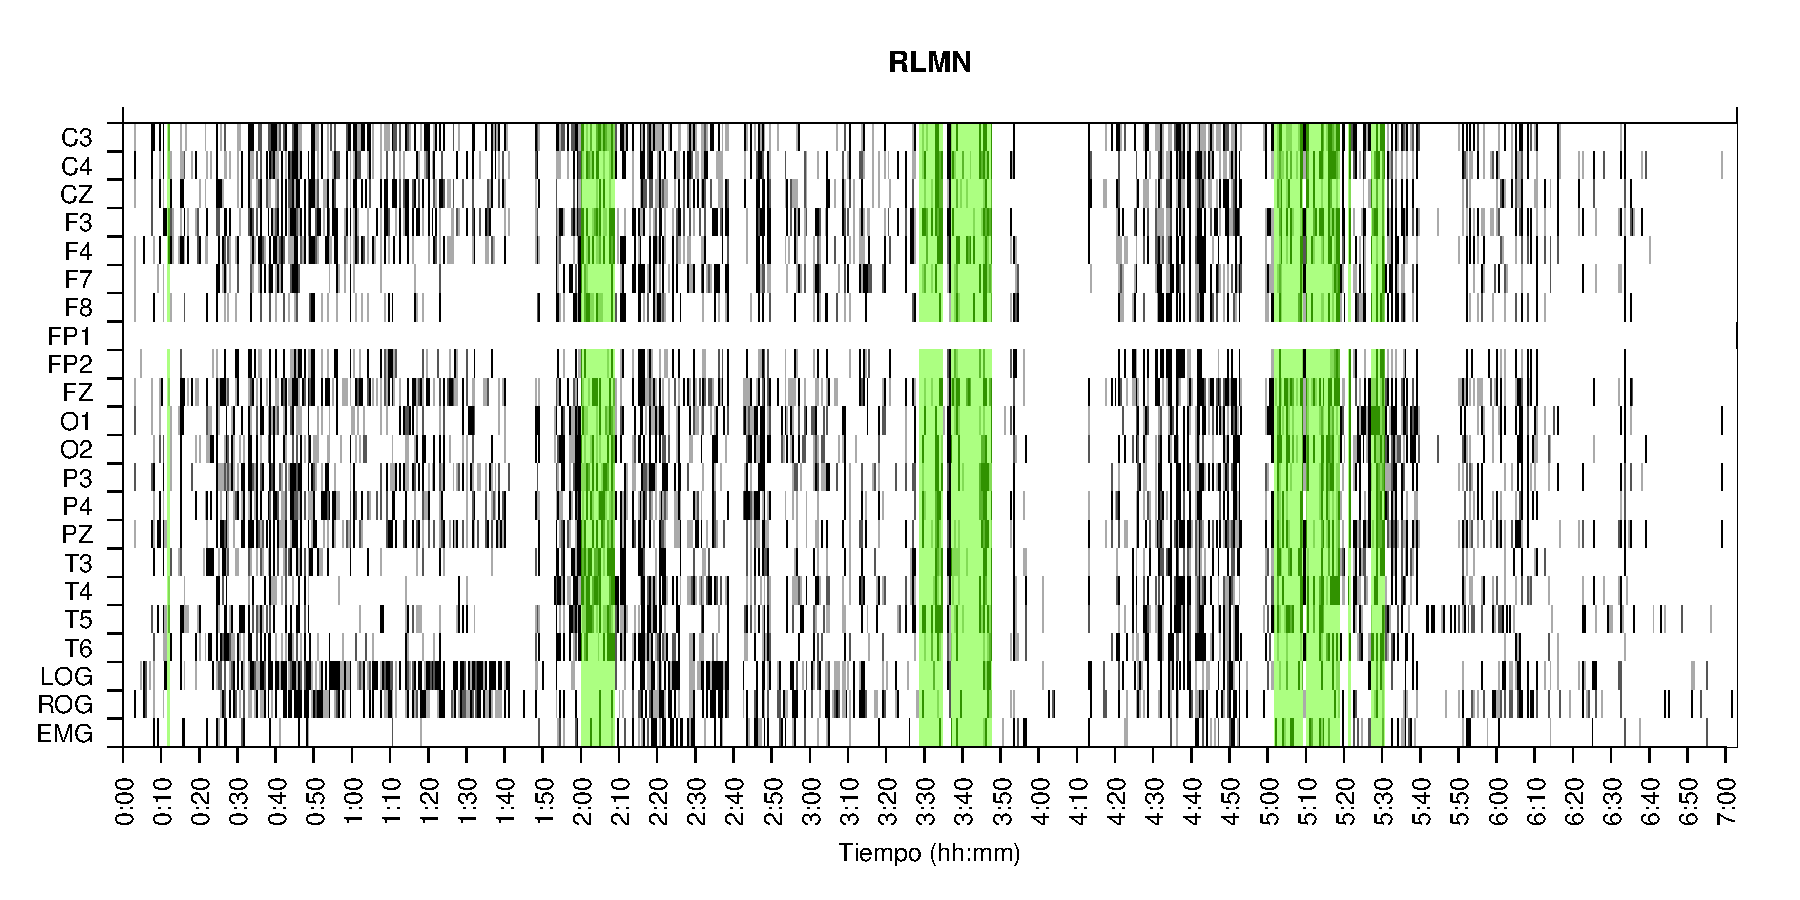
\includegraphics[width=\linewidth]{./material_bonito170220/RLMN10SUE_99_mor99_tot846_est_total.pdf} 
%\caption{Sujeto: RLMN | Total \'epocas: 846 | \'Epocas MOR: 99}
%%\label{primera}
%\end{SidewaysFigure}
%\begin{SidewaysFigure}
%\centering
%\includegraphics[width=\linewidth]
%{./material_bonito170220/RLMN10SUE_99_mor99_tot99_est_mor.pdf} 
%\caption{Sujeto: RLMN | \'Epocas MOR: 99 | (\'Unicamente \'epocas MOR)}
%%\label{primera}
%\end{SidewaysFigure}
%
%\begin{figure}
%\centering
%\includegraphics[width=\linewidth]
%{./material_bonito170220/porcentaje_bis/RLMN10SUE_99_846_1_bar_porcentaje.pdf} 
%\caption{Sujeto: RLMN | Porcentaje de \'epocas \textit{posiblemente estacionarias}}
%\end{figure}
%
%%%%%%%%%%%%%%%%%%%%%%%%%%%%%%%%%%%%
%%%%%%%%%%%%%%%%%%%%%%%%%%%%%%%%%%%%
%
%\begin{SidewaysFigure}
%\centering
%\includegraphics[width=\linewidth]
%{./material_bonito170220/JANASUE_103_mor103_tot907_est_total.pdf} 
%\caption{Sujeto: JANA | Total \'epocas: 907 | \'Epocas MOR: 103}
%%\label{primera}
%\end{SidewaysFigure}
%\begin{SidewaysFigure}
%\centering
%\includegraphics[width=\linewidth]
%{./material_bonito170220/JANASUE_103_mor103_tot103_est_mor.pdf} 
%\caption{Sujeto: JANA | \'Epocas MOR: 103 | (\'Unicamente \'epocas MOR)}
%%\label{primera}
%\end{SidewaysFigure}
%
%\begin{figure}
%\centering
%\includegraphics[width=\linewidth]
%{./material_bonito170220/porcentaje_bis/JANASUE_103_907_1_bar_porcentaje.pdf} 
%\caption{Sujeto: JANA | Porcentaje de \'epocas \textit{posiblemente estacionarias}}
%\end{figure}
%
%%%%%%%%%%%%%%%%%%%%%%%%%%%%%%%%%%%%
%%%%%%%%%%%%%%%%%%%%%%%%%%%%%%%%%%%%
%
%\begin{SidewaysFigure}
%\centering
%\includegraphics[width=\linewidth]
%{./material_bonito170220/CLMN10SUE_132_mor132_tot944_est_total.pdf} 
%\caption{Sujeto: CLMN | Total \'epocas: 944 | \'Epocas MOR: 132}
%%\label{primera}
%\end{SidewaysFigure}
%\begin{SidewaysFigure}
%\centering
%\includegraphics[width=\linewidth]
%{./material_bonito170220/CLMN10SUE_132_mor132_tot132_est_mor.pdf} 
%\caption{Sujeto: CLMN | \'Epocas MOR: 132 | (\'Unicamente \'epocas MOR)}
%%\label{primera}
%\end{SidewaysFigure}
%
%\begin{figure}
%\centering
%\includegraphics[width=\linewidth]
%{./material_bonito170220/porcentaje_bis/CLMN10SUE_132_944_1_bar_porcentaje.pdf} 
%\caption{Sujeto: CLMN | Porcentaje de \'epocas \textit{posiblemente estacionarias}}
%\end{figure}
%
%%%%%%%%%%%%%%%%%%%%%%%%%%%%%%%%%%%%
%%%%%%%%%%%%%%%%%%%%%%%%%%%%%%%%%%%%
%
%\begin{SidewaysFigure}
%\centering
%\includegraphics[width=\linewidth]
%{./material_bonito170220/CLMN10SUE_132_mor132_tot944_est_total.pdf} 
%\caption{Sujeto: JGMN | Total \'epocas: 1207 | \'Epocas MOR: 33}
%%\label{primera}
%\end{SidewaysFigure}
%\begin{SidewaysFigure}
%\centering
%\includegraphics[width=\linewidth]
%{./material_bonito170220/JGMN6SUE_33_mor33_tot33_est_mor.pdf} 
%\caption{Sujeto: CLMN | \'Epocas MOR: 33 | (\'Unicamente \'epocas MOR)}
%%\label{primera}
%\end{SidewaysFigure}
%
%\begin{figure}
%\centering
%\includegraphics[width=\linewidth]
%{./material_bonito170220/porcentaje_bis/JGMN6SUE_33_1207_1_bar_porcentaje.pdf} 
%\caption{Sujeto: JGMN | Porcentaje de \'epocas \textit{posiblemente estacionarias}}
%\end{figure}
%
%%%%%%%%%%%%%%%%%%%%%%%%%%%%%%%%%%%%
%%%%%%%%%%%%%%%%%%%%%%%%%%%%%%%%%%%%
%
%\begin{SidewaysFigure}
%\centering
%\includegraphics[width=\linewidth]
%{./material_bonito170220/RRMNS_114_mor114_tot1244_est_total_bis.pdf} 
%\caption{Sujeto: RRMN | Total \'epocas: 1244 | \'Epocas MOR: 114}
%%\label{primera}
%\end{SidewaysFigure}
%\begin{SidewaysFigure}
%\centering
%\includegraphics[width=\linewidth]
%{./material_bonito170220/RRMNS_114_mor114_tot114_est_mor_bis.pdf} 
%\caption{Sujeto: RRMN | \'Epocas MOR: 114 | (\'Unicamente \'epocas MOR)}
%%\label{primera}
%\end{SidewaysFigure}
%
%\begin{figure}
%\centering
%\includegraphics[width=\linewidth]
%{./material_bonito170220/porcentaje_bis/RRMNS_114_1244_1_bar_porcentaje.pdf} 
%\caption{Sujeto: RRMN | Porcentaje de \'epocas \textit{posiblemente estacionarias}}
%\end{figure}
%
%%%%%%%%%%%%%%%%%%%%%%%%%%%%%%%%%%%%
%%%%%%%%%%%%%%%%%%%%%%%%%%%%%%%%%%%%
%
%\begin{SidewaysFigure}
%\centering
%\includegraphics[width=\linewidth]
%{./material_bonito170220/VCNNS1_200_mor200_tot2584_est_total.pdf} 
%\caption{Sujeto: VCNN | Total \'epocas: 2586 | \'Epocas MOR: 200}
%%\label{primera}
%\end{SidewaysFigure}
%\begin{SidewaysFigure}
%\centering
%\includegraphics[width=\linewidth]
%{./material_bonito170220/VCNNS1_200_mor200_tot200_est_mor.pdf} 
%\caption{Sujeto: VCNN | \'Epocas MOR: 200 | (\'Unicamente \'epocas MOR)}
%%\label{primera}
%\end{SidewaysFigure}
%
%\begin{figure}
%\centering
%\includegraphics[width=\linewidth]
%{./material_bonito170220/porcentaje_bis/VCNNS1_200_2584_1_bar_porcentaje.pdf} 
%\caption{Sujeto: VCNN | Porcentaje de \'epocas \textit{posiblemente estacionarias}}
%\end{figure}
%
%%%%%%%%%%%%%%%%%%%%%%%%%%%%%%%%%%%%
%%%%%%%%%%%%%%%%%%%%%%%%%%%%%%%%%%%%
%
%\begin{SidewaysFigure}
%\centering
%\includegraphics[width=\linewidth]
%{./material_bonito170220/FGHSUE_22_mor22_tot405_est_total.pdf} 
%\caption{Sujeto: FGH | Total \'epocas: 405 | \'Epocas MOR: 22}
%%\label{primera}
%\end{SidewaysFigure}
%\begin{SidewaysFigure}
%\centering
%\includegraphics[width=\linewidth]
%{./material_bonito170220/FGHSUE_22_mor22_tot22_est_mor.pdf} 
%\caption{Sujeto: FGH | \'Epocas MOR: 22 | (\'Unicamente \'epocas MOR)}
%%\label{primera}
%\end{SidewaysFigure}
%
%\begin{figure}
%\centering
%\includegraphics[width=\linewidth]
%{./material_bonito170220/porcentaje_bis/FGHSUE_22_405_1_bar_porcentaje.pdf} 
%\caption{Sujeto: FGH | Porcentaje de \'epocas \textit{posiblemente estacionarias}}
%\end{figure}
%
%%%%%%%%%%%%%%%%%%%%%%%%%%%%%%%%%%%%
%%%%%%%%%%%%%%%%%%%%%%%%%%%%%%%%%%%%
%
%\begin{SidewaysFigure}
%\centering
%\includegraphics[width=\linewidth]
%{./material_bonito170220/GH24031950SUENO_267_mor267_tot3281_est_total.pdf} 
%\caption{Sujeto: GURM | Total \'epocas: 3281 | \'Epocas MOR: 267}
%%\label{primera}
%\end{SidewaysFigure}
%\begin{SidewaysFigure}
%\centering
%\includegraphics[width=\linewidth]
%{./material_bonito170220/GH24031950SUENO_267_mor267_tot267_est_mor.pdf} 
%\caption{Sujeto: GURM | \'Epocas MOR: 267 | (\'Unicamente \'epocas MOR)}
%%\label{primera}
%\end{SidewaysFigure}
%
%\begin{figure}
%\centering
%\includegraphics[width=\linewidth]
%{./material_bonito170220/porcentaje_bis/GH24031950SUENO_267_3281_1_bar_porcentaje.pdf} 
%\caption{Sujeto: GURM | Porcentaje de \'epocas \textit{posiblemente estacionarias}}
%\end{figure}

%%%%%%%%%%%%%%%%%%%%%%%%%%%%%%%%%%%
%%%%%%%%%%%%%%%%%%%%%%%%%%%%%%%%%%%

%%%%%%%%%%%%%%%%%%%%%%%%%%%%%%%%%%%%%%%%%%%%%%%%%%%%%%%%%%%%%%%%%%%%%%%%%%%%%%%%%%%%%%%%%%%%%%%%%%%
%%%%%%%%%%%%%%%%%%%%%%%%%%%%%%%%%%%%%%%%%%%%%%%%%%%%%%%%%%%%%%%%%%%%%%%%%%%%%%%%%%%%%%%%%%%%%%%%%%%